\chapter{Fundamental Architecture}
Dopo aver analizzato nel dettaglio i meccanismi del Cloud Computing passiamo alle architetture fondamentali, che essenzialmente hanno come obiettivo quello di essere una rappresentazione formale dei domini funzionali, cioè un'astrazione delle richieste, requisiti e risposte ai requisiti specifici del dominio di applicazione. I meccanismi visti finora rappresentano dei building block che vengono messi insieme per costruire delle architetture che sono le soluzioni che specificano le interazioni, i comportamenti e le combinazioni tra meccanismi. 

\section{Workload Distribution}
Come sappiamo le risorse IT possono scalare orizzontalmente attraverso una quantità di risorse identiche replicate, e con un load balancer con una logica a runtime che decide di distribuire in maniera equa il carico attraverso le risorse. Come sappiamo serve ad evitare errori di sovrautilizzo e viene applicato ad ogni risorsa (non solo ai server). Ci sono versioni specializzate che riguardano server load balancing e switch virtuali, in quanto anche la rete può scalare. 

\begin{figure}[htb!]
    \centering
    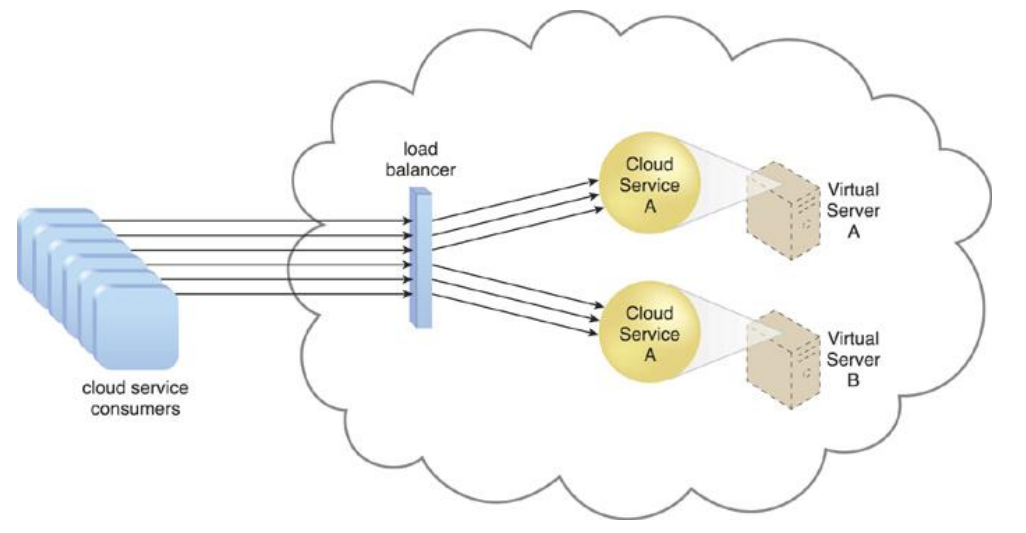
\includegraphics[width=10cm]{./Images/cap11/11.1.png}
\end{figure}

In questo scenario i meccanismi che usiamo sono:
\begin{itemize}
    \item Load balancer
    \item Virtual server
    \item Cloud storage device
    \item Audit monitor: serve per poter monitorare i log, gli accessi in modo da poter fornire certificazione e documentazione degli utenti che hanno compiuto operazioni, ma anche per controllare l'aspetto regolatorio del servizio che viene fornito, definito nel SLA.
    \item Cloud usage monitor, per capire quante risorse vengono adoperate per fornire il servizio in maniera scalabile.
    \item Hypervisor, perché il meccanismo comporta l'uso delle macchine virtuali.
    \item Logical Network Perimeter: è necessario l'isolamento dei livelli dove i carichi di lavoro sono distribuiti.
    \item Resource Cluster: per supportare il balancing.
\end{itemize}

\section{Resource Pooling}
I pool di risorse mettono a disposizione una serie di risorse di base, che sono:
\begin{itemize}
    \item server fisici, cioè server che vengono considerati insieme un'unica risorsa e possono essere utilizzati in maniera comune coordinata.
    \item server virtuali, più semplici da gestire in quanto esistono dei template.
    \item storage pool: cioè un'insieme di risorse di storage che vengono allocate in caso di necessità.
    \item Network: risorse di rete fornite con caratteristiche come ridondanza e link aggregation, tramite il quale diversi link fisici vengono usati come un unico link "virtuale" che ha come larghezza di banda la somma delle larghezze di banda dei singoli link.
    \item CPU: tipicamente si hanno più core o processori virtuali e non singoli processori standard.
    \item memoria: anche la RAM viene messa insieme in pool di risorse.
\end{itemize}
Questi pool possono essere messi insieme oppure possono essere isolati, o innestati, rappresentando un partizionamento. L'obiettivo di questo partizionamento si può vedere dall'immagine: le richieste inviate al pool A.1 non possono eccedere le risorse del pool A.1, e stessa cosa vale per il pool A.2.

\begin{figure}[htb!]
    \centering
    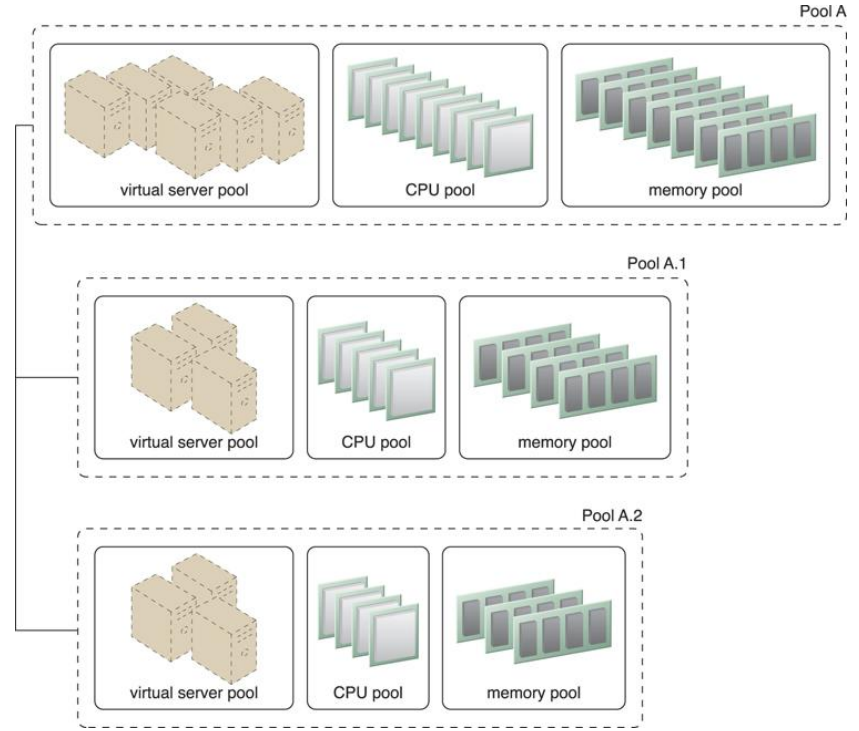
\includegraphics[width=9cm]{./Images/cap11/11.2.png}
\end{figure}

I meccanismi utilizzati sono:
\begin{itemize}
    \item Virtual server
    \item Cloud storage device
    \item Audit Monitor: per monitorare l'utilizzo per le regolazioni dei dati e anche per la privacy.
    \item Cloud Usage Monitor, per capire quanto pagare per un pool di risorse.
    \item Hypervisor
    \item Logical Network Perimeter
    \item Pay-Per-Use Monitor, per tariffare l'utilizzo di risorse nel pool: trasforma le risorse in denaro per il provider.
    \item Remote Administration Systems (per i soldi)
    \item Resource Administration System (per le risorse)
    \item Resource replication
\end{itemize}

\section{Dynamic Scalability}
La scalabilità dinamica è sia molto utile che pericoloso perché può porre problemi sotto una determinata configurazione durante un attacco DoS. Funziona facendo il trigger per l'allocazione delle risorse in base a condizioni predefinite senza alcun intervento manuale: riesce quindi a mantenere le prestazioni del servizio e la QoS all'interno dei termini specificati nel SLA allocando le risorse automaticamente in base alle fluttuazioni del carico. Il vantaggio è che non richiede intervento umano, lo svantaggio è che può portare a costi imprevisti in caso di picchi non prevedibili.

Lo scaling viene effettuato in tre modi:
\begin{itemize}
    \item \textbf{Dynamic Horizontal Scaling} - classico scaling orizzontale che fa scaling out e scaling in, l'Automated Scaling Listener segnala che è necessario replicare le risorse.
    \item \textbf{Dynamic Vertical Scaling} - classico scaling verticale che fa scaling up e scaling down, l'Automated Scaling Listener segnala che è necessario aumentare le risorse che vengono date alle macchine.
    \item \textbf{Dynamic Relocation} - l'istanza del servizio viene spostata verso un host che ha maggiore capacità. La differenza principalmente è che mentre nei due precedenti parliamo di istanze virtuali, qui si parla di istanze fisiche.
\end{itemize}

I meccanismi utilizzati sono:
\begin{itemize}
    \item Automated Scaling Listener (fondamentale)
    \item Resource Replication (anch'esso fondamentale)
    \item Cloud Usage Monitor, per loggare l'utilizzo di nuove risorse o di risorse più potenti.
    \item Hypervisor
    \item Pay-Per-Use Monitor
\end{itemize}

\section{Elastic Resource Capacity}
Tipicamente legata alla fornitura di server virtuali (con CPU e RAM), l'interazione è tipicamente con l'hypervisor o con la VIM per ottenere le risorse che vengono elasticamente aggiunte a quello che viene fornito al customer. In questa struttura è importante anticipare le richieste, prima che si arrivi a una thresold fissata. Una componente automatica, chiamata \textit{intelligent automation engine} manda le scaling requests alla VIM oppure direttamente all'hypervisor, e in certi casi è necessario il reboot della risorsa. È tipico del modello di deployment IaaS. Nella figura è mostrato il funzionamento: all'aumentare dei cloud service consumer, l'intelligent automation engine usa degli script comunicando all'hypervisor la necessità di aumentare le risorse per la macchina virtuale (scaling verticale).

\begin{figure}[htb!]
    \centering
    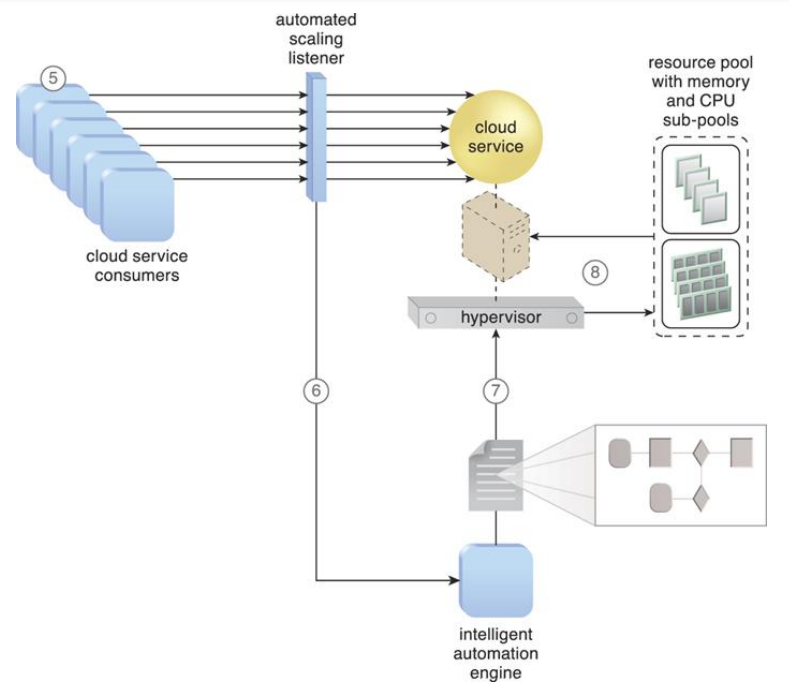
\includegraphics[width=9cm]{./Images/cap11/11.3.png}
\end{figure}

I meccanismi utilizzati sono:
\begin{itemize}
    \item Cloud Usage Monitor
    \item Pay-Per-Use Monitor, che raccoglie i costi dello scaling.
    \item Resource Replication
\end{itemize}

\section{Service Load Balancing}
Permette il bilanciamento dei servizi, ed è tipico del modello di deployment SaaS. Può essere considerato una variazione della workload distribution architecture, ma per far scalare le implementazioni dei servizi cloud. Si basa su una serie di implementazioni duplicate del servizio da bilanciare: un load balancer quindi è esterno a queste implementazioni, oppure può essere il servizio stesso ad applicare politiche di bilanciamento (ovviamente solo in senso orizzontale). 
La figura mostra le due possibili implementazioni: nello scenario A il load balancer è indipendente dal servizio, nello scenario B è il servizio stesso a bilanciare il carico. Lo scenario A può essere più semplice da implementare ma può avere degli svantaggi nel caso ci siano bilanciamenti molto precisi da fare, in quanto essendo indipendente dal servizio non ne conosce l'implementazione e non può ottimizzarne le prestazioni, cosa che è possibile nello scenario B.

\begin{figure}[htb!]
    \centering
    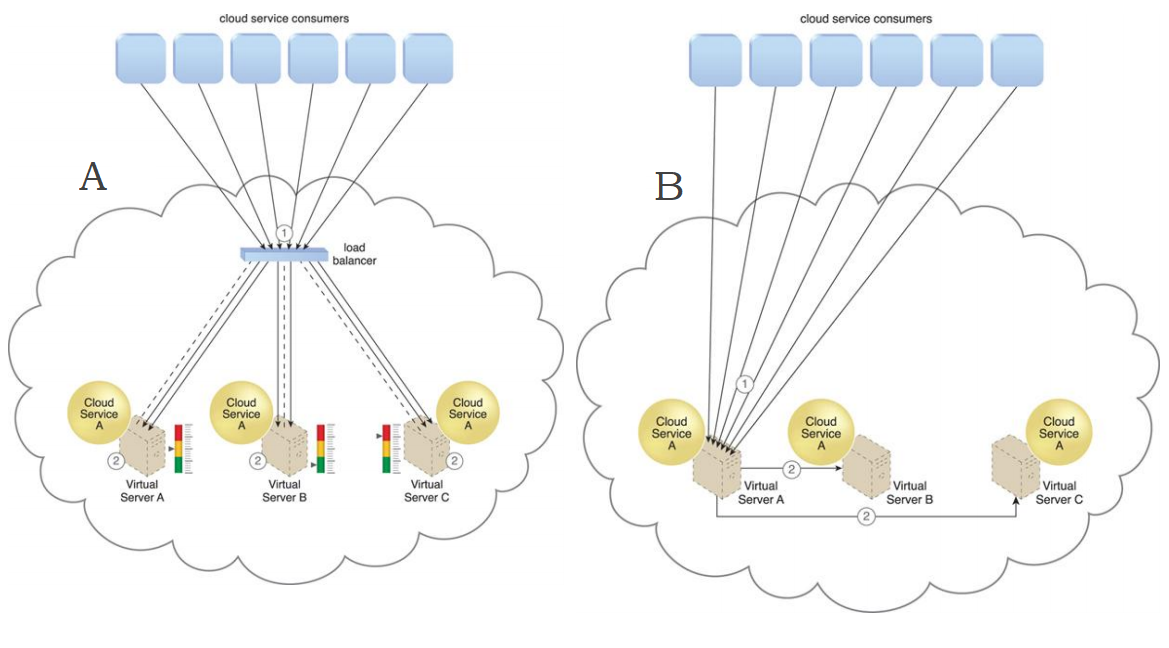
\includegraphics[width=13cm]{./Images/cap11/11.4.png}
\end{figure}

I meccanismi utilizzati sono:
\begin{itemize}
    \item Cloud Usage Monitor
    \item Resource Cluster
    \item Resource Replication
\end{itemize}

\section{Cloud Bursting}
Questo meccanismo stabilisce una forma di scaling dinamico che scala o "fa esplodere" una risorsa IT on-premise sul cloud quando è necessario, e questo può accadere per motivi politici, logistici o economici. In breve, l'utilizzo della risorsa potrebbe essere basso per cui può restare on premise, ma se dovesse aumentare questo meccanismo permette di spostarla su cloud in maniera agile. Questo avviene anche al contrario, ovvero quando non è più necessaria, la risorsa torna nell'ambiente on-premise. Ovviamente questo meccanismo richiede che siano utilizzati un Automated Scaling Listener e un meccanismo di Resource Replication.

\begin{figure}[htb!]
    \centering
    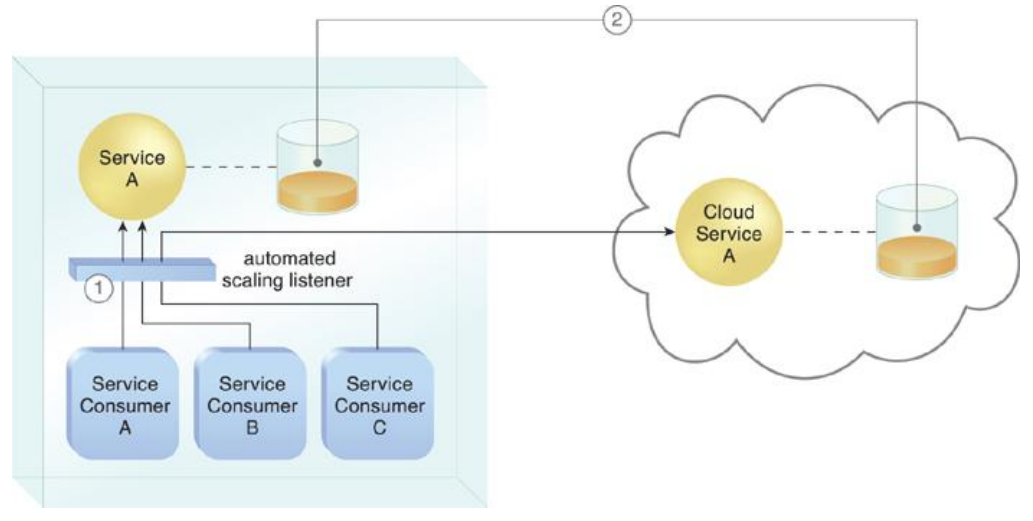
\includegraphics[width=9cm]{./Images/cap11/11.5.png}
\end{figure}

Come si può vedere dalla figura, un ASL verifica costantemente l'utilizzo del cloud service A e nel caso in cui venga superata una certa soglia, le richieste vengono redirette su un'istanza perfettamente identica (grazie allo state replication) sul cloud.

\section{Elastic Disk Provisioning}
Permette di utilizzare taglie variabili di storage, basandosi ovviamente su dischi virtuali, per offrire una fatturazione più granulare. Grazie all'allocazione dinamica inoltre spesso la maggior parte delle spese non vengono affrontate perché il consumer viene addebitato solo per ciò che effettivamente usa.

I meccanismi utilizzati sono:
\begin{itemize}
    \item Cloud Storage Device
    \item Virtual Server
    \item Hypervisor
    \item Pay-per-use monitor
    \item Cloud usage monitor
    \item Resource replication, usato per convertire i diversi tipi di elastic disk provisioning.
\end{itemize}

\section{Redundant Storage}
La ridondanza dello storage è utile per offrire alta disponibilità, resilienza, e tolleranza ai fallimenti. Un \textbf{LUN} (Logical Unit Number), visto anche in precedenza, è un disco logico che rappresenta una partizione di un disco fisico. Lo \textbf{Storage Service Gateway} è una componente che si comporta come un dispositivo di storage ma non fa il gateway verso dischi fisici. Tipicamente per favorire il Redundant Storage si definisce una replica dello storage per poter gestire i fallimenti: in caso di fallimenti del nodo tutte le richieste vengono redirette verso la copia. 

\begin{figure}[htb!]
    \centering
    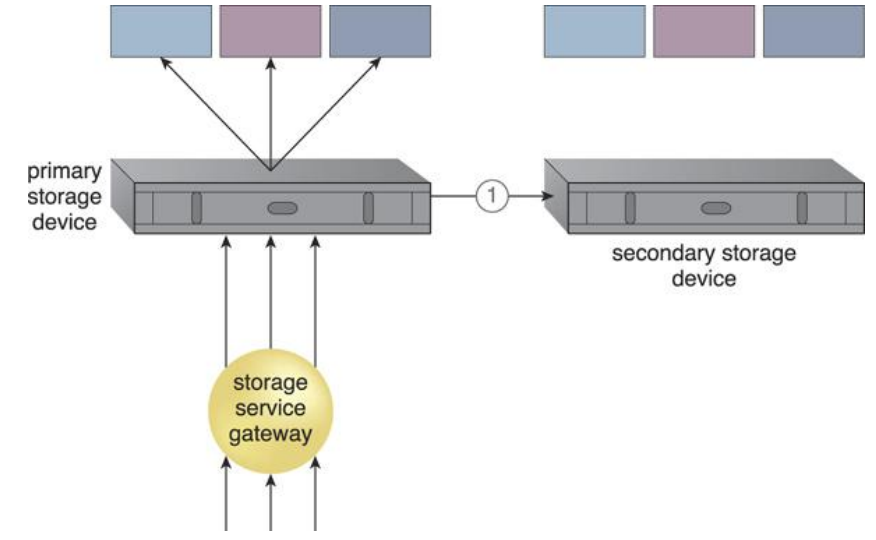
\includegraphics[width=9cm]{./Images/cap11/11.6.png}
\end{figure}

Lo Storage Service Gateway fornisce accesso al primary storage device, che però mantiene automaticamente duplicato il suo stato, quindi ogni LUN viene replicata nel nuovo storage. In caso di fallimenti o malfunzionamenti del primary storage, il SSG switcha automaticamente sul secondary storage device.

Per risparmiare, i cloud providers potrebbero localizzare i cloud storage secondari in regioni geografiche differenti dal primary storage, e dunque sorgono i tipici problemi del data residency sui tipi di dati che vengono salvati che possono portare anche a problemi legali. Per questo i protocolli e i metodi utilizzati per lo scambio di messaggi e per la sincronizzazione tra lo storage primario e quello secondario devono supportare crittografia e meccanismi di sicurezza avanzati per poter supportare la QoS dei dati che sono stati duplicati in un altro contesto. Ovviamente, anche i protocolli di replica potrebbero essere soggetti a restrizioni dovute alle diverse zone geografiche. 

La replica dello storage in differenti aree geografiche viene utilizzata anche per supportare il disaster recovery.

\section{Learning Check}
\begin{enumerate}
    \item Descrivi l'obiettivo dell'architettura di Workload Distribution e spiega come viene utilizzato il Load Balancer in relazione ad essa. Inoltre elenca i meccanismi del Cloud Computing utilizzati in questa architettura.
    \item Descrivi l'obiettivo dell'architettura di Resource Pooling ed elenca i tipi comuni di risorse che possono essere raggruppate. Elenca i tre tipi principali di gruppi di resource pool e spiegane le gerarchie. Inoltre elenca i meccanismi del Cloud Computing utilizzati in questa architettura.
    \item Descrivi l'obiettivo dell'architettura Dynamic Scalability e spiega come questa è in relazione con le condizioni di scaling predefinite e con il meccanismo di Automated Scaling Listener. Inoltre elenca i meccanismi del Cloud Computing utilizzati in questa architettura.
    \item Descrivi l'obiettivo dell'architettura Elastic Resource Capacity e spiegane l'utilizzo in relazione ai resource pool e a un sistema di elastic provisioning. Inoltre elenca i meccanismi del Cloud Computing utilizzati in questa architettura.
    \item Descrivi l'obiettivo dell'architettura Service Load Balancing. Inoltre elenca i meccanismi del Cloud Computing utilizzati in questa architettura.
    \item Descrivi l'obiettivo dell'architettura Cloud Bursting e spiega come vengono utilizzati i meccanismi di Automated Scaling Listener e Resource Replication. Inoltre illustra la differenza tra un'architettura che effettua un \textit{burst} verso un cloud pubblico rispetto ad un cloud privato.
    \item Descrivi l'obiettivo dell'architettura Elastic Disk Provisioning e spiega come viene utilizzato insieme al Dynamic Storage Provisioning System. Inoltre elenca i meccanismi del Cloud Computing utilizzati in questa architettura.
    \item Descrivi l'obiettivo dell'architettura Redundant Storage e spiega come storage primario e storage secondario vengono utilizzati in un Failover System. Inoltre elenca i meccanismi del Cloud Computing utilizzati in questa architettura.
\end{enumerate}
